\documentclass[12pt]{article}

\usepackage{amsmath}
\usepackage{amsfonts}
\usepackage{amssymb}
\usepackage{graphicx}
\usepackage[center]{caption}
\usepackage{mathtools}
\usepackage{lipsum}
\usepackage{stackengine}
\usepackage{fancyhdr}
\usepackage{caption}
\usepackage{tikz}
\usetikzlibrary{shapes.geometric, arrows}
\usepackage{float}
\usepackage[a4paper,left=1in,right=1in,top=1in,bottom=1in,footskip=.25in]{geometry}
\usepackage{etoolbox}
\usepackage[nottoc]{tocbibind}
\usepackage{tabu}
\usepackage{enumitem,kantlipsum}
\usepackage{verbatim}
\usepackage{hyperref}
\begin{document}


\section{Aim}
This test case is for checking the capability of the written Isogeometric analysis code of a 2D Piezoelectric plate under electrical loading
\section{Problem description} \label{2DPPWEL}
\emph{Section 7.4.1 in Documentation}\\
A 2D piezoelectric plate subjected to electrical loading is considered, as shown in Fig. (\ref{PureElectrical}) . The material used is PZT-PIC151 ceramics.

\begin{figure}[H]
	\centering
	\begin{minipage}{.5\textwidth}
		\centering
		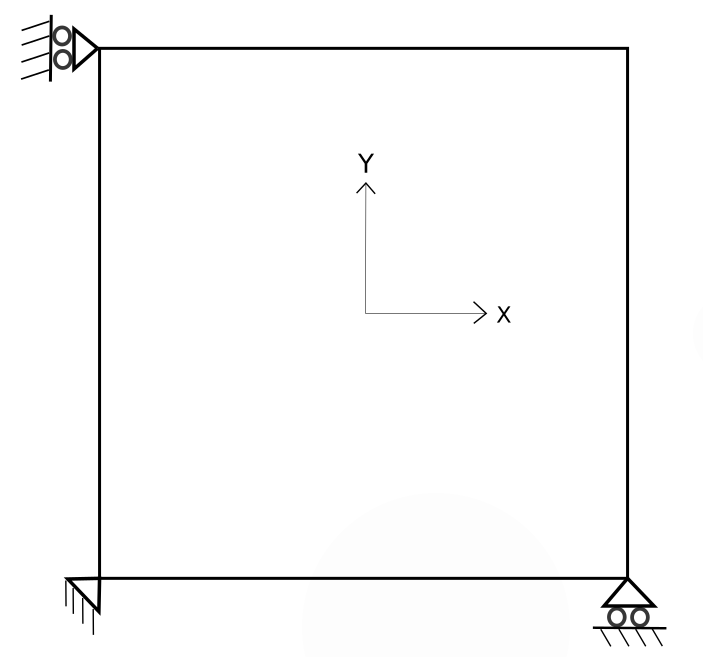
\includegraphics[width=0.8\linewidth]{2DPlate.png}
		\captionof{figure}{2D Piezoelectric Plate}
		\label{2Dplate}
	\end{minipage}%
	\begin{minipage}{.4\textwidth}
		\centering
		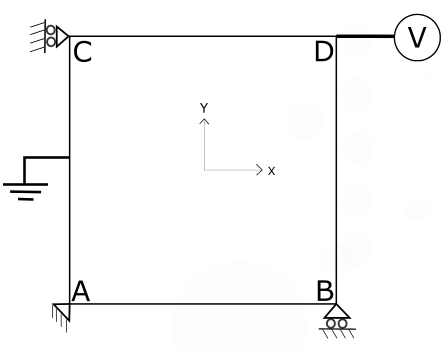
\includegraphics[width=1\linewidth]{PureElectrical.png}
		\captionof{figure}{2D Piezoelectric Plate with loading}
		\label{PureElectrical}
	\end{minipage}
\end{figure}
The movement of the bottom edge AB and left edge AC of 2D piezoelectric plate is fixed in y-direction and x-direction respectively, as shown in figure(\ref{PureElectrical}).
The top edge CD is grounded (Electric potential $\Phi = 0$), and an electrical potential of 100 V  is applied on the bottom edge AB. The results for a single element case and multiple elements are discussed in the below
sections. \\
The results generated by IGA code are compared with inbuilt Abaqus piezoelectric
element \textbf{CPE4E}.

\newpage

\section{How to run the Program}
\begin{enumerate}[leftmargin=*]
	\item The code is written in python and external libraries numpy, matplotlib.pyplot, sys, path from pathlib and math are used.
	\item Please use any environment which will compile python programs
	\item Place all the files in a single folder.
	\item A file named Input.py can be edited to change the dimensions of the plate. User can change Length, Height and Thickness of the plate. \\(The results discussed below are for Length = 10 mm, Height = 10 mm and Thickness = 1 mm)
	\begin{figure}[H]
		\begin{center}
			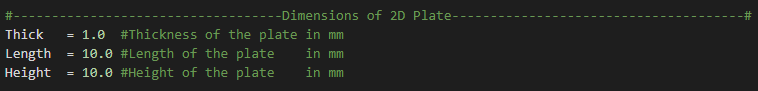
\includegraphics[scale=0.8]{Input.png} 
		\end{center}	
	\end{figure}
	\item Before you run the file, please make sure that the working directory is same as the folder  which
	Consists the Program.
	\item Use command  $>>>$ python Main\_Program.py to run the program.
	\item The contour plots will be saved in the folder \textbf{Results.}
	\item A "log.txt" file is created in the same folder which contains the values of the results plotted.
	
	
\end{enumerate}

\newpage

\section{Results and discussions}
\emph{Section 7.4.3 in Documentation}\\
Abaqus plane strain full integration piezoelectric element (\textbf{CPE4E}) is used for analysis. The below figures show the values of displacements (U), electrical potentials (EPOT) and the reactive electrical nodal charge (RCHG) for both Abaqus and IGA element.\\

Figure(\ref{EME1U1}) and Figure(\ref{EME1U1_IGA}) show the displacement (U1) values of the single CPE4E element and single IGA element at 100 \% loading in x-direction respectively. \\
\begin{figure}[H]
	\centering
	\begin{minipage}{.5\textwidth}
		\centering
		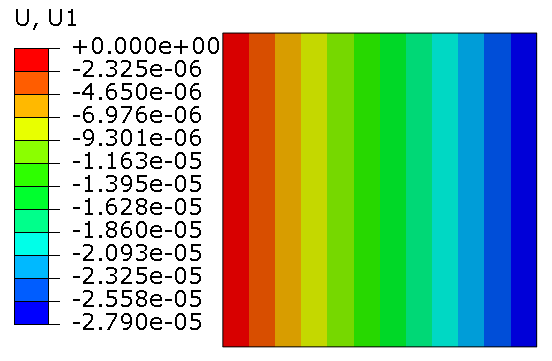
\includegraphics[width=1\linewidth]{EME1U1.png}
		\captionof{figure}{CPE4E Element:U1
			\\\textbf{Abaqus generated result}}
		\label{EME1U1}
	\end{minipage}%
	\begin{minipage}{.55\textwidth}
		\centering
		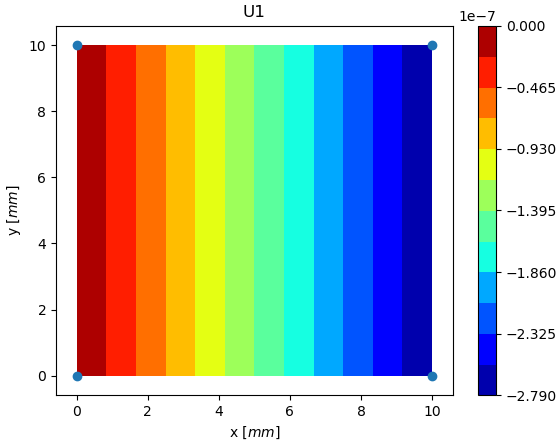
\includegraphics[width=1\linewidth]{EME1U1_IGA.png}
		\captionof{figure}{IGA Piezoelectric Element:U1\\ \textbf{Program generated result}}
		\label{EME1U1_IGA}
	\end{minipage}
\end{figure}
\noindent
Figure(\ref{EME1U2}) and Figure(\ref{EME1U2_IGA}) show the displacement (U2) values of the single CPE4E element and single IGA element at 100 \% loading in y-direction respectively. \\
\begin{figure}[H]
	\centering
	\begin{minipage}{.5\textwidth}
		\centering
		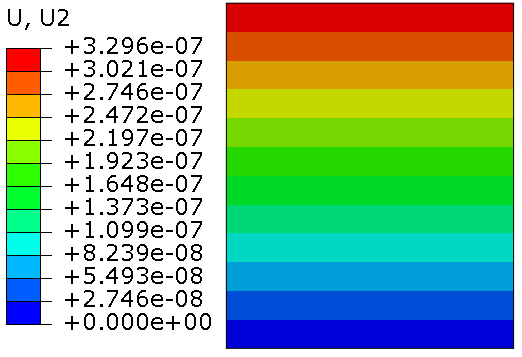
\includegraphics[width=1\linewidth]{EME1U2.png}
		\captionof{figure}{CPE4E Element:U2
			\\\textbf{Abaqus generated result}}
		\label{EME1U2}
	\end{minipage}%
	\begin{minipage}{.55\textwidth}
		\centering
		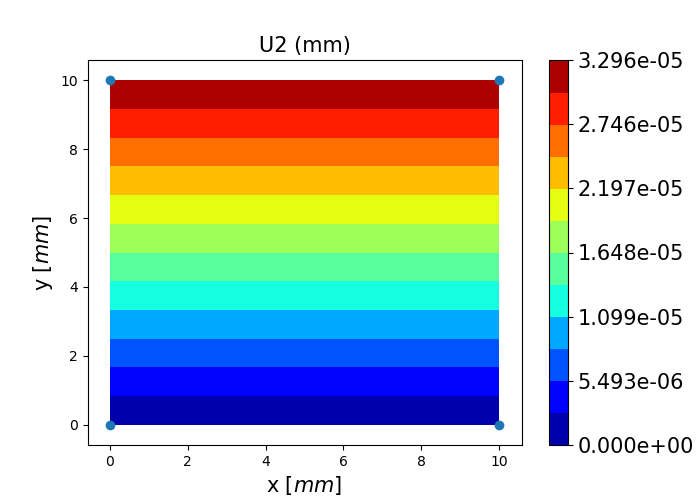
\includegraphics[width=1\linewidth]{EME1U2_IGA.png}
		\captionof{figure}{IGA Piezoelectric Element:U2\\ \textbf{Program generated result}}
		\label{EME1U2_IGA}
	\end{minipage}
\end{figure}
\begin{comment}
\begin{figure}[H]
\begin{center}
\includegraphics[scale=0.45]{xyz.png} 
\caption{\\CPE4 Element U1}\label{xyz}
\end{center}	
\end{figure}

\begin{figure}[H]
\begin{center}
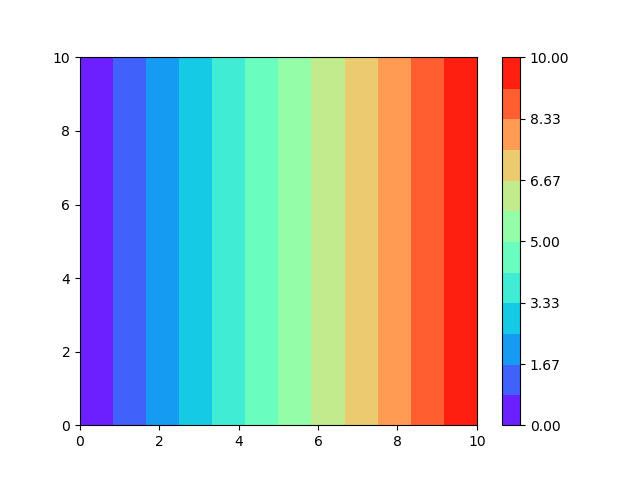
\includegraphics[scale=0.8]{Figure_1.png} 
\caption{\\IGA Element U1}\label{Figure_1}
\end{center}	
\end{figure}
\end{comment}


Figure(\ref{EME1EPOT}) and Figure(\ref{EME1EPOT_IGA}) show the Electrical potential values (EPOT) of the single CPE4E element and single IGA element at 100 \% loading respectively. \\
\begin{figure}[H]
	\centering
	\begin{minipage}{.5\textwidth}
		\centering
		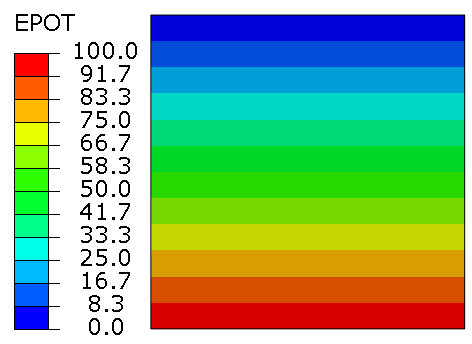
\includegraphics[width=1\linewidth]{EME1EPOT.png}
		\captionof{figure}{CPE4E Element:EPOT
			\\\textbf{Abaqus generated result}}
		\label{EME1EPOT}
	\end{minipage}%
	\begin{minipage}{.6\textwidth}
		\centering
		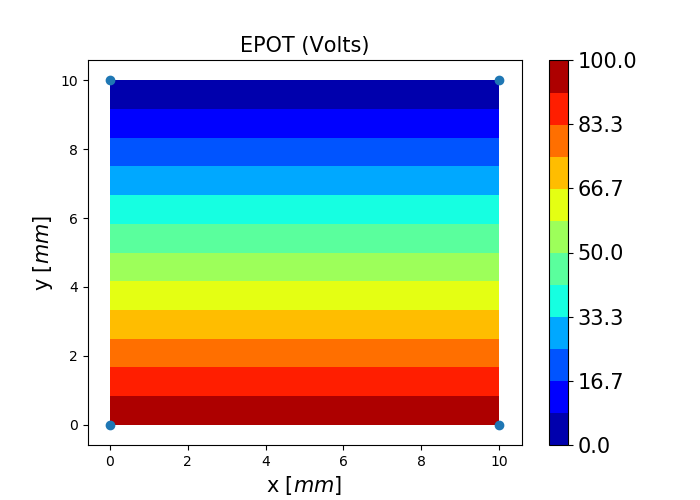
\includegraphics[width=1\linewidth]{EME1EPOT_IGA.png}
		\captionof{figure}{IGA Piezoelectric Element:EPOT\\ \textbf{Program generated result}}
		\label{EME1EPOT_IGA}
	\end{minipage}
\end{figure}

Figure(\ref{EME1RCHG}) and Figure(\ref{EME1RCHG_IGA}) show the Reactive electrical nodal charge (RCHG) of the single CPE4E element and single IGA element at 100 \% loading respectively. \\
\begin{figure}[H]
	\centering
	\begin{minipage}{.5\textwidth}
		\centering
		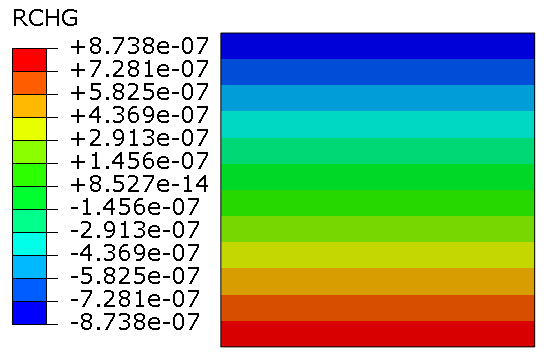
\includegraphics[width=1\linewidth]{EME1RCHG.png}
		\captionof{figure}{CPE4E Element:RCHG
			\\\textbf{Abaqus generated result}}
		\label{EME1RCHG}
	\end{minipage}%
	\begin{minipage}{.6\textwidth}
		\centering
		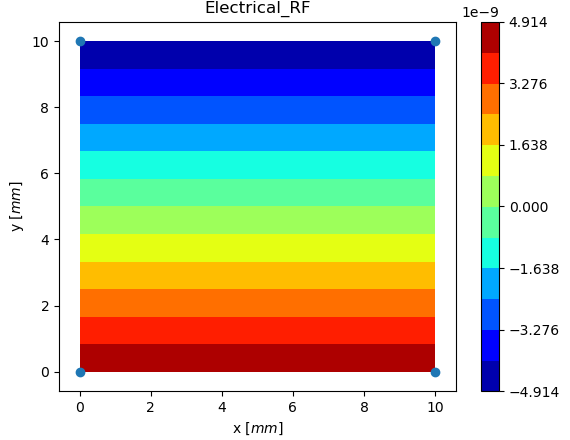
\includegraphics[width=1\linewidth]{EME1RCHG_IGA.png}
		\captionof{figure}{IGA Piezoelectric Element:RCHG\\ \textbf{Program generated result}}
		\label{EME1RCHG_IGA}
	\end{minipage}
\end{figure}


\end{document}